\documentclass[11pt]{article}

\usepackage[a4paper,margin=2.45cm]{geometry}
\usepackage[T1]{fontenc}
\usepackage[utf8]{inputenc}
\usepackage{lmodern}
\usepackage{amsmath,amssymb}
\usepackage{booktabs,threeparttable,longtable,array,tabularx}
\usepackage{graphicx,float}
\usepackage{caption,subcaption}
\usepackage{setspace}
\usepackage{xcolor}
\usepackage{enumitem}
\usepackage{microtype}
\usepackage[colorlinks=true,linkcolor=black,citecolor=black,urlcolor=blue]{hyperref}
\usepackage[backend=biber,style=authoryear-comp,maxcitenames=2,maxbibnames=99,uniquelist=false]{biblatex}
\addbibresource{green_credit_transition_refs.bib}

\captionsetup{font=small,labelsep=quad}
\setlength{\tabcolsep}{4pt}
\renewcommand{\arraystretch}{1.13}
\onehalfspacing
\setlist{nosep,leftmargin=2em}
\setlength{\emergencystretch}{2em}

\newcommand{\note}[1]{\begin{minipage}{0.96\textwidth}\footnotesize\textit{Notes:} #1\end{minipage}}

\title{Green Credit and the Limits of Transition in Coal-Intensive Regions:\\
Evidence from Continuous Coal Exposure and Provincial Pathways in China}
\author{Sihan Wang \and Yiran Liu \and Manyu Lou \and Youen Zhao}
\date{}

\begin{document}
\maketitle

\begin{abstract}
This study asks which margins of adjustment changed more strongly in coal-intensive Chinese provinces after the 2012 Green Credit Guidelines, and whether those changes extended from the operation of the existing energy system to its capital and generation structure. We interact a post-2012 indicator with provinces' average coal share in five categories of final energy consumption during 2008--2011 and estimate continuous-exposure difference-in-differences models on a provincial panel. In the baseline estimates, provinces with greater pre-policy coal exposure experienced larger post-2012 declines in final-energy intensity, final-coal intensity, industrial sulfur dioxide, nitrogen oxides, industrial solid waste emissions, and the coal share of energy use. The coal-share outcome provides the clearest pre-policy dynamic evidence. The intensity and pollution estimates, however, are sensitive to differential trends, and an observable green-credit proxy does not validate a distinct financial transmission channel. These estimates therefore document differential post-policy changes consistent with stronger constraints on coal-intensive activity, rather than an isolated causal effect of the Green Credit Guidelines. Carbon dioxide emissions and the thermal capacity and generation shares did not exhibit stable contemporaneous differences. An index of the early clean-power base, constructed from pre-policy nonthermal capacity and 2013--2016 wind capacity and generation, did not consistently amplify later renewable substitution; negative triple interactions may also reflect convergence and limited remaining growth space. A comparison of Shanxi and Inner Mongolia reveals robust differences in policy attention to green finance and clean coal, but not in pollution-control or renewable-energy topics. The evidence points to a hierarchy of adjustment: operating intensity and the composition of energy use moved first, while the replacement of energy capital and generation structures was slower and more dependent on local conditions. Green credit is best understood as one external financial constraint on coal-intensive development, not as a policy instrument sufficient to complete structural substitution on its own.

\noindent\textbf{Keywords:} green credit; coal exposure; energy intensity; carbon lock-in; regional endowments; policy text

\noindent\textbf{JEL codes:} Q48; Q52; Q56; G21; R11
\end{abstract}

\section{Introduction}

Green investment is constrained by environmental externalities, asymmetric information, and long payback periods. When pollution costs are not fully incorporated into private decisions, markets undervalue the social return to cleaner investment \parencite{pigou1920}. Banks may also ration credit because they cannot perfectly identify borrowers' environmental risk or the quality of transition projects \parencite{stiglitzweiss1981}. In bank-based financial systems, incorporating environmental and social risk into lending standards can therefore complement price-based environmental regulation \parencite{campiglio2016,dikauvolz2021}. China's banking regulator issued the Green Credit Guidelines in 2012, requiring banks to embed environmental and social risk in pre-lending review, credit approval, contract design, and post-lending management, with differentiated treatment of energy-intensive, polluting, and excess-capacity industries \parencite{cbrc2012}.

Research on China's green-credit regime has examined corporate finance, green innovation, environmental performance, and carbon emissions. Early studies traced the transition from broad policy commitments to bank-level procedures \parencite{aizawayang2010,zhangyangbi2011}. Later work documented changes in financing costs, debt maturity, investment, and bank risk \parencite{cuietal2018,xuli2020}. Recent quasi-experimental studies report effects on corporate carbon intensity, pollution, environmental performance, renewable investment, and green innovation, although the direction and channels vary across ownership, financing constraints, regulatory environments, and firm capabilities \parencite{heetal2019,xuyetal2023,wuetal2023,zhangetal2024green,laietal2024,lietal2024,pengetal2024,machen2025,zhengetal2025,zhangetal2025micro}. This literature establishes that green credit can alter firm behavior. It says less about which layer of a coal-intensive regional energy system adjusts first.

That distinction matters. Coal-intensive regions can comply with tighter financing and environmental requirements by reducing energy input per unit of output, curtailing high-emission activity, or installing treatment equipment without immediately retiring coal and thermal-power capital. Even a decline in coal's share of final energy can reflect growth in gas, electricity, or other energy carriers rather than the retirement of thermal assets. Large energy assets are long-lived, partly irreversible, and embedded in complementary networks and institutions. These features generate technological and institutional lock-in \parencite{arthur1989,david1985,unruh2000}. A financial constraint may thus change operating margins before it changes the reproduction of the energy system.

Local energy conditions complicate this sequence. Classic resource economics explains how exhaustible-resource stocks shape extraction and investment paths \parencite{hotelling1931}, while the resource-curse literature links resource dependence to industrial concentration, fiscal dependence, and institutional incentives \parencite{auty1993,sachswarner2001}. Yet wind and solar resources, or an early clean-power base, are opportunities rather than sufficient conditions for transition. Converting an external policy signal into new industries and projects requires related knowledge, absorptive capacity, infrastructure, and policy coordination \parencite{cohenlevinthal1990,hidalgoetal2007,neffkeetal2011,boschma2017,hansencoenen2015}. Neither coal abundance nor an early wind-power base uniquely determines the regional response.

We therefore ask a layered question. After 2012, on which margins did provinces with greater pre-policy coal exposure change more strongly? Did those changes extend from operating intensity and emissions to the composition of energy use, carbon emissions, and thermal-power structure? Did an early clean-power base or resource dependence systematically alter that extension? We assemble a provincial panel for 2000--2023, interact a post-2012 indicator with pre-policy final-coal exposure, and combine the baseline comparison with continuous-exposure event studies, alternative exposures, province-specific trends, an observable green-credit proxy, resource-dependence measures, and policy texts from Shanxi and Inner Mongolia.

The study makes three contributions. First, it separates \textbf{operational adjustment}, \textbf{compositional adjustment}, and \textbf{structural substitution}. This ordering follows from adjustment costs and asset irreversibility: inputs and emissions can change relatively quickly; coal's share of energy use is an intermediate margin; thermal capital and renewable project systems adjust more slowly. Second, it connects green-credit research to the literature on regional endowments and path dependence. The analysis tests whether a national financial constraint is associated with different layers of change across coal exposure and the early clean-power base, without equating existing wind capacity with a complete measure of local capability. Third, the paper reports identification limits directly. The supplemental diagnostics reveal pre-policy differences in core intensity outcomes and substantial sensitivity to province-specific trends, while the observable green-credit proxy does not establish a clear policy channel. The paper accordingly contributes a hierarchy of post-policy facts and a boundary argument, not a strong claim that one national policy caused every observed change.

\section{Literature Review and Conceptual Framework}

\subsection{Green credit as environmental regulation through capital allocation}

Environmental economics begins with the divergence between private and social marginal costs \parencite{pigou1920}. Taxes, standards, and emissions trading internalize this divergence through prices or quantities. Green credit adds a capital-allocation mechanism. Under asymmetric information, banks clear credit markets not only through interest rates but also through loan amounts, maturity, covenants, and access \parencite{stiglitzweiss1981}. Once regulators require banks to recognize environmental risks, pollution records and industry classifications can alter borrower screening, risk assessment, and monitoring. Green credit therefore combines financing with the financial enforcement of environmental regulation \parencite{campiglio2016,dikauvolz2021}.

The literature on China yields three broad sets of findings. The first concerns institutional implementation. \textcite{aizawayang2010} and \textcite{zhangyangbi2011} emphasize that green credit depends not only on the amount of preferential funding but also on whether environmental information enters lending procedures. The second concerns financial outcomes. Green lending may be associated with bank risk \parencite{cuietal2018}, while the Guidelines changed debt costs and maturity asymmetrically for polluting firms \parencite{xuli2020}. The third examines real behavior. Studies document changes in renewable investment, corporate carbon intensity, innovation, and environmental performance \parencite{heetal2019,xuyetal2023,wuetal2023}. Research published in 2024--2025 extends these findings to pollution treatment, green transformation, financial resilience, and heterogeneous firm responses \parencite{zhangetal2024green,laietal2024,lietal2024,pengetal2024,machen2025,zhengetal2025,zhangetal2025micro}.

Firm-level effectiveness does not imply simultaneous provincial energy restructuring. Firms can respond through output contraction, input substitution, mature abatement equipment, or project reclassification. These responses are generally faster and less capital intensive than building renewable plants, connecting them to the grid, and retiring thermal assets. A regional test must therefore distinguish the margin on which an effect appears.

\subsection{Adjustment costs, induced innovation, and structural substitution}

The effect of environmental regulation on productivity has long been organized around compliance costs and innovation compensation. The Porter hypothesis proposes that well-designed regulation can induce innovation and partly offset compliance costs \parencite{portervanderlinde1995}. Evidence on research and patenting, however, does not imply immediate productivity gains \parencite{jaffepalmer1997}. Models of induced innovation and directed technical change show that relative prices and policy incentives redirect technological search, but the existing knowledge stock makes the response path dependent \parencite{popp2002,acemogluetal2012,aghionetal2016}. Renewable-energy patent responses also vary by technology and policy instrument \parencite{johnstoneetal2010}.

These theories imply an adjustment hierarchy. We define \textbf{operational adjustment} as changes within the existing coal-intensive system, including final-energy intensity, final-coal intensity, and pollutant emissions. \textbf{Compositional adjustment} is a change in coal's relative share of energy use. \textbf{Structural substitution} is a sustained reorganization of thermal capital, generation, carbon trajectories, and renewable project systems. Operational adjustment does not require asset retirement; compositional adjustment can arise from several energy quantities moving simultaneously; structural substitution requires new capital formation, network access, and the retirement or repurposing of old capital. Financial constraints should therefore appear first on operational margins, while structural variables respond more slowly and conditionally.

\subsection{Local energy endowments, lock-in, and regional capabilities}

Exhaustible resources shape regional industrial, fiscal, and employment structures \parencite{hotelling1931,auty1993,sachswarner2001}. Once coal mining, thermal generation, transport networks, and local public finance become complementary, increasing returns and coordination costs reinforce the incumbent path \parencite{arthur1989,david1985,unruh2000}. Sustainability-transition research accordingly treats technological substitution as the co-evolution of technologies, markets, infrastructure, and institutions \parencite{geels2002,markardetal2012}. Regional pathways differ because knowledge bases, industrial relatedness, and policy capacities differ \parencite{hansencoenen2015,boschma2017}.

Absorptive-capacity theory argues that the use of external knowledge depends on prior knowledge and organizational capability \parencite{cohenlevinthal1990}. Product-space and regional-relatedness studies likewise show that regions diversify more easily into activities related to existing capabilities \parencite{hidalgoetal2007,neffkeetal2011}. Green technological diversification exhibits the same dependence; political support operates through, rather than independently of, local knowledge and industrial conditions \parencite{santoalhaboschma2021}. Recent studies show that the relationship between resource dependence and renewable development can be nonlinear and policy dependent \parencite{zhangetal2024resource}; that brown regions' entry into green technologies depends on economic strength and knowledge combinations \parencite{grashofbasilico2025}; and that coal-region transitions must address employment, public finance, and regional justice \parencite{healybarry2017,carleyetal2018,demeterova2024,tassikittner2024,perettoetal2025}. New work on regional absorptive capacity similarly interprets policy outcomes as the joint product of external intervention and local technological foundations \parencite{zhaoetal2026}.

This literature rejects two deterministic claims. Resource abundance need not make green policy ineffective because infrastructure, technical skills, and resource revenues may be redeployed. A strong wind or solar base also need not produce faster subsequent growth because high initial levels, grid constraints, and project cycles can restrict marginal expansion. We therefore label our index an \emph{early clean-power base}, not a natural-resource endowment or a complete measure of regional capability.

\subsection{Research gap and empirical expectations}

Green-credit studies focus primarily on corporate finance and environmental outcomes; regional-transition studies focus on resource dependence, technological relatedness, and local capabilities. Three gaps remain at their intersection. First, there is little integrated evidence on which layer of a coal-intensive regional system responds first to a national financial regulation. Second, the broad label ``green transition'' often obscures whether a lower coal share is accompanied by changes in carbon emissions, thermal capital, and thermal generation. Third, it remains unclear whether an existing clean-power base is sufficient to translate tighter financial constraints into later renewable substitution.

We derive three bounded empirical expectations. First, after 2012, provinces with higher pre-policy coal exposure may exhibit larger declines in operating intensity and selected pollutant emissions. Second, coal's share may decline without synchronous changes in the variables that represent deep structural substitution. Third, the sign of the interaction between coal exposure and the early clean-power base is theoretically ambiguous: first-mover advantages can coexist with convergence, grid constraints, and limited remaining growth space. These expectations organize the evidence but do not turn a statistically insignificant estimate into proof of no effect.

\section{Institutional Background, Data, and Research Design}

\subsection{Institutional setting and object of identification}

The Green Credit Guidelines were issued in February 2012. They required banks to identify, measure, monitor, and control environmental and social risks, and to adjust approval, contracts, and post-lending management according to the nature and severity of those risks \parencite{cbrc2012}. Because the policy applied nationally, there is no naturally untreated province. We use pre-policy coal exposure as a measure of potential treatment intensity. Provinces where coal represented a larger share of final energy were generally more connected to regulated coal-intensive activities and may therefore have faced a stronger post-policy financing and compliance constraint.

This design identifies \textbf{differential post-2012 changes} across provinces with different pre-policy coal exposure. It does not observe the amount by which banks tightened or expanded green credit. Energy-conservation targets, coal-consumption controls, air-pollution policies, supply-side reforms, and provincial industrial policies also changed after 2012 and may have affected coal provinces differentially. Province and year fixed effects cannot absorb such concurrent exposure-specific policies. We therefore treat the continuous DID as a main post-policy comparison and use event studies, differential trends, alternative exposures, and an observable green-credit proxy to assess its credibility.

\subsection{Sample and data sources}

The base panel contains 31 mainland Chinese provincial units from 2000 through 2023, yielding 744 province-year observations. Controls such as environmental fiscal expenditure and the marketization index have more complete coverage from 2007, so most main regressions use 2007--2023; the five-energy variables end in 2022. Each table reports its actual sample size.

Macroeconomic variables come from the \emph{China Statistical Yearbook} and National Bureau of Statistics provincial series compiled through Wind. Energy variables come from provincial energy-balance tables in the \emph{China Energy Statistical Yearbook} and corresponding Wind exports. The five energy categories are coal, petroleum products, liquefied petroleum gas, natural gas, and electricity. They do not exhaust all primary energy, so we consistently use the term ``five-energy measure.'' Physical quantities are converted to ten thousand tons of standard coal equivalent using consistent coefficients and aggregated. Power capacity and generation come from the \emph{China Electric Power Statistical Yearbook} and Wind provincial series. Emissions come from the \emph{China Environment Statistical Yearbook} and official ecological-environment statistics. Provincial CO$_2$ is aggregated from EDGAR 2024 (v8.0) gridded fossil-fuel and industrial-process emissions and measured in tons \parencite{crippaetal2024}.

The supplementary green-credit measure is drawn from the user-provided workbook \emph{Green Credit Level, 2005--2022}, which covers 31 provinces. Its underlying series is the share of interest expenses paid by six energy-intensive industries in the interest expenses of above-scale industrial firms. We construct a positively signed proxy:
\begin{equation}
\begin{aligned}
\text{Green-credit proxy}_{it}
=1-\frac{\text{Interest expense of six energy-intensive industries}_{it}}
{\text{Interest expense of above-scale industrial firms}_{it}}.
\end{aligned}
\end{equation}
A higher value indicates a lower share of industrial interest expenses paid by energy-intensive industries. This is a financing-structure proxy, not the regulatory balance of provincial green loans. The source workbook interpolates 2017; the supplementary estimates are therefore also reported without that year.

The policy-text corpus consists of public documents from the Shanxi and Inner Mongolia government websites. After cleaning, it contains 3,874 Shanxi documents and 2,974 Inner Mongolia documents for 2000--2023. We combine title, subject, and body text, count dictionaries for green finance, clean coal, pollution control, and renewable energy, and construct occurrences per 10,000 Chinese characters and the share of documents mentioning each topic at least once. Dictionary counts do not identify semantic direction, and historical archiving differs between websites. The measures capture policy attention, not policy-support intensity.

\subsection{Variable construction and conceptual mapping}

Pre-policy coal exposure is the 2008--2011 mean share of coal in final consumption of the five energy categories:
\begin{equation}
\begin{aligned}
\text{Coal exposure}_{i}
=\frac{1}{4}\sum_{s=2008}^{2011}
\frac{\text{Final coal consumption}_{is}}
{\text{Final consumption of five energy categories}_{is}}.
\end{aligned}
\end{equation}
The provincial mean is 0.415, the standard deviation is 0.149, and the range is 0.102--0.644. The main regressor is Post-2012 $\times$ Coal exposure. The exposure level is time invariant and absorbed by province fixed effects.

Operational outcomes include final consumption of the five energy categories divided by GDP, final coal consumption divided by GDP, and industrial SO$_2$, NO$_x$, and solid-waste emissions. The project does not contain a complete provincial GDP deflator, so the intensity measures use nominal GDP. We additionally estimate log energy quantities conditional on GDP. Green total factor productivity (GTFP) and the global Malmquist--Luenberger (GML) index are inherited variables whose underlying input, desirable-output, and undesirable-output files are unavailable for complete reconstruction. They are retained as supplementary outcomes but do not carry the main conclusion.

Compositional outcomes are the coal share in the five-energy measure and the original statistical coal-consumption share. Structural outcomes include log CO$_2$ emissions, thermal capacity and generation shares, nonthermal generation, wind generation, wind-plus-solar generation, and wind capacity. Table \ref{tab:mapping} maps the conceptual hierarchy to the empirical measures.

\begin{table}[H]
\centering
\caption{Adjustment hierarchy and empirical measures}
\label{tab:mapping}
\begin{tabularx}{\textwidth}{p{3.1cm}p{4.0cm}X p{2.6cm}}
\toprule
Layer & Concept & Measures & Evidentiary role \\
\midrule
Operational: intensity & Lower inputs within the incumbent energy system & Five-energy final intensity; final-coal intensity & Baseline evidence; dynamic and trend sensitive \\
Operational: emissions & Joint changes in polluting activity, output, and treatment & Industrial SO$_2$, NO$_x$, solid waste; PM and wastewater & Baseline evidence; does not isolate end-of-pipe treatment \\
Compositional & Change in coal's relative share of energy use & Five-energy coal share; original coal-consumption share & Clearest dynamic evidence \\
Structural: deep & Joint reorganization of thermal capital, generation, and carbon path & CO$_2$; thermal capacity and generation shares & Boundary evidence; thermal generation has a pre-trend \\
Structural: renewable & Expansion of renewable capacity, generation, and projects & Nonthermal, wind, and wind-solar generation; wind capacity & Exploratory conditional evidence \\
Local pathways & Local policy agendas and ex post energy outcomes & Shanxi--Inner Mongolia text measures and period means & Descriptive case evidence \\
\bottomrule
\end{tabularx}
\end{table}

The early clean-power base is the mean of three standardized components: the 2008--2011 nonthermal capacity share, the 2013--2016 wind-capacity share, and the 2013--2016 wind-generation share:
\begin{equation}
\begin{aligned}
\text{Early clean-power base}_{i}=\frac{1}{3}\big[&z(\text{pre-policy nonthermal capacity}_{i})
+z(\text{early wind capacity}_{i})\\
&+z(\text{early wind generation}_{i})\big].
\end{aligned}
\end{equation}
Because the latter two components occur after 2012, this index is not a strictly exogenous pre-policy endowment. It describes clean-power infrastructure formed by 2016. The resource-dependence index is the mean of standardized pre-policy mining employment, coal-mining assets, and resource-tax dependence; a four-component version adds coal-output dependence.

\subsection{Econometric specifications}

The baseline two-way fixed-effects model is
\begin{equation}
\begin{aligned}
Y_{it}={}&\beta(\text{Post-2012}_{t}\times\text{Coal exposure}_{i})
+\gamma'X_{it}+\mu_i+\lambda_t+\varepsilon_{it},
\end{aligned}
\label{eq:did}
\end{equation}
where $X_{it}$ includes log provincial GDP, population, the secondary-industry share, urbanization, the environmental-fiscal-expenditure share, and the marketization index. Province and year fixed effects are denoted by $\mu_i$ and $\lambda_t$. Standard errors are clustered by province. The coefficient $\beta$ is a post-policy difference associated with a one-unit increase in pre-policy coal exposure, not the effect of a one-unit increase in green lending.

The continuous-exposure event study uses 2011 as the omitted year and pools 2008 and earlier and 2016 and later:
\begin{equation}
\begin{aligned}
Y_{it}={}&\sum_{\tau\neq -1}\beta_{\tau}
\left(\text{Coal exposure}_{i}\times\mathbf{1}[t-2012=\tau]\right)\\
&+\gamma'X_{it}+\mu_i+\lambda_t+\varepsilon_{it}.
\end{aligned}
\label{eq:event}
\end{equation}
Joint tests of the pre-policy coefficients assess differential trends. Because the main regression window begins in 2007, the earliest bin contains only a limited number of years.

For renewable outcomes, we use a post-2016 indicator and retain every identifiable lower-order interaction:
\begin{equation}
\begin{aligned}
Y_{it}={}&\beta_1(\text{Post-2016}_{t}\times\text{Coal exposure}_{i})\\
&+\beta_2(\text{Post-2016}_{t}\times\text{Early clean base}_{i})\\
&+\theta(\text{Post-2016}_{t}\times\text{Coal exposure}_{i}
\times\text{Early clean base}_{i})\\
&+\gamma'X_{it}+\mu_i+\lambda_t+\varepsilon_{it}.
\end{aligned}
\label{eq:ddd}
\end{equation}
The time-invariant Coal exposure $\times$ Early clean base term is absorbed by province fixed effects. The coefficient $\theta$ indicates whether the combination of coal exposure and an early clean-power base is associated with a different post-2016 change; it cannot isolate resource, project, or grid channels.

The Shanxi--Inner Mongolia text specification is a two-province fixed-effects comparison based on Inner Mongolia $\times$ Post-2012. With only two provinces and different website archives, it is descriptive rather than causal.

\section{Empirical Results}

\subsection{Descriptive statistics}

Table \ref{tab:desc} summarizes the main variables. Coal exposure has a province-year mean of 0.415 and a standard deviation of 0.147. The energy-intensity outcomes display substantial variation. Wind and wind-solar outcomes are more complete only from 2011, so their effective samples are smaller. The green-credit proxy covers 2005--2022 and 558 province-years.

\begin{table}[H]
\centering
\caption{Descriptive statistics}
\label{tab:desc}
\begin{tabular}{lrrrrr}
\toprule
Variable & Obs. & Mean & Std. dev. & Min. & Max. \\
\midrule
Pre-policy coal exposure & 720 & 0.415 & 0.147 & 0.102 & 0.644 \\
Five-energy final intensity & 686 & 0.650 & 0.428 & 0.088 & 4.726 \\
Final-coal intensity & 686 & 0.285 & 0.287 & 0.001 & 3.221 \\
Industrial SO$_2$ & 720 & 45.203 & 39.481 & 0.059 & 171.500 \\
NO$_x$ & 348 & 53.057 & 39.522 & 3.490 & 180.110 \\
Industrial solid waste & 720 & 40.002 & 33.608 & 0.158 & 160.500 \\
Five-energy coal share & 686 & 0.379 & 0.167 & 0.007 & 0.746 \\
Log CO$_2$ emissions & 744 & 19.077 & 0.915 & 16.081 & 20.887 \\
Thermal capacity share & 683 & 0.652 & 0.241 & 0.024 & 1.000 \\
Thermal generation share & 735 & 0.716 & 0.255 & 0.001 & 1.000 \\
Wind-solar generation share & 342 & 0.075 & 0.076 & 0.000 & 0.447 \\
Green-credit proxy & 558 & 0.460 & 0.147 & 0.094 & 0.972 \\
\bottomrule
\end{tabular}
\end{table}

\subsection{Operational adjustment: energy intensity and pollutant emissions}

The first test asks whether post-2012 differences appear on operating margins within the incumbent energy system. Table \ref{tab:intensity} reproduces the baseline estimates. The coefficient on Post-2012 $\times$ Coal exposure is $-0.2895$ for five-energy final intensity and $-0.4262$ for final-coal intensity, significant at the 5 and 1 percent levels. Multiplying by the provincial standard deviation of coal exposure, 0.149, gives changes of approximately $-0.043$ and $-0.064$ sample units. GTFP and the GML index are statistically insignificant. The evidence therefore points to lower measured energy-input intensity in the baseline specification, not a general green-productivity increase.

\begin{table}[H]
\centering
\caption{Post-policy coal exposure and energy intensity}
\label{tab:intensity}
\resizebox{0.96\textwidth}{!}{%
\begin{tabular}{lcccc}
\toprule
 & GTFP & Global ML index & Five-energy final intensity & Final-coal intensity \\
\midrule
Post-2012 $\times$ Coal exposure & -1.0498 & -0.1342 & -0.2895** & -0.4262*** \\
 & (0.7528) & (0.0830) & (0.1190) & (0.0776) \\
Observations & 510 & 510 & 480 & 480 \\
$R^2$ & 0.7644 & 0.2719 & 0.9592 & 0.9237 \\
Province/year fixed effects & Yes & Yes & Yes & Yes \\
\bottomrule
\end{tabular}}
\note{Province-clustered standard errors in parentheses. ***, **, and * denote significance at 1, 5, and 10 percent. GTFP and GML are inherited outcomes that cannot be fully reconstructed from the available source files and are supplementary.}
\end{table}

The second operational test concerns pollutant emissions. In Table \ref{tab:pollution}, the coefficients for industrial SO$_2$, NO$_x$, and industrial solid waste are $-72.5887$, $-43.9915$, and $-47.2683$, respectively, and statistically significant. Particulate matter and industrial wastewater are insignificant. These outcomes are emissions, so a decline may arise from output contraction, relocation, fuel substitution, or end-of-pipe treatment. The estimates support a bounded claim about pollutant-emission responses; they do not isolate higher pollution-control investment.

\begin{table}[H]
\centering
\caption{Post-policy coal exposure and pollutant-emission responses}
\label{tab:pollution}
\resizebox{\textwidth}{!}{%
\begin{tabular}{lccccc}
\toprule
 & Industrial SO$_2$ & NO$_x$ & Particulates & Industrial solid waste & Industrial wastewater \\
\midrule
Post-2012 $\times$ Coal exposure & -72.5887*** & -43.9915** & -10.1339 & -47.2683** & -40594.6149 \\
 & (19.6996) & (16.8916) & (28.0627) & (20.0521) & (24203.0698) \\
Observations & 510 & 336 & 154 & 510 & 510 \\
$R^2$ & 0.8812 & 0.9223 & 0.8225 & 0.7837 & 0.9108 \\
Province/year fixed effects & Yes & Yes & Yes & Yes & Yes \\
\bottomrule
\end{tabular}}
\note{Province-clustered standard errors are in parentheses. Lower emissions alone do not identify an end-of-pipe abatement channel.}
\end{table}

\subsection{Compositional adjustment and the boundary of structural substitution}

The next test asks whether the post-policy differences extend from operating margins to energy composition and deeper structural outcomes. Table \ref{tab:structure} places these outcomes side by side. The coefficients for the five-energy coal share and the original coal-consumption share are $-0.2495$ and $-0.1900$, both significant at 1 percent. The coefficients for CO$_2$, thermal capacity, and thermal generation are statistically insignificant. A lower coal share is therefore evidence of compositional adjustment, but it does not by itself demonstrate thermal-system exit. Nor do the insignificant estimates prove zero effects: the 95 percent confidence interval for log CO$_2$ is approximately $[-0.310,0.113]$, and the intervals for the thermal shares are also wide.

\begin{table}[H]
\centering
\caption{Coal-use composition, carbon emissions, and thermal structure}
\label{tab:structure}
\resizebox{\textwidth}{!}{%
\begin{tabular}{lccccc}
\toprule
 & Five-energy & Original & Log CO$_2$ & Thermal capacity & Thermal generation \\
 & coal share & coal share & emissions & share & share \\
\midrule
Post-2012 $\times$ Coal exposure & -0.2495*** & -0.1900*** & -0.0982 & 0.0517 & 0.0888 \\
 & (0.0754) & (0.0651) & (0.1034) & (0.0945) & (0.0754) \\
Observations & 480 & 480 & 510 & 510 & 507 \\
$R^2$ & 0.9224 & 0.9382 & 0.9904 & 0.9368 & 0.9478 \\
Province/year fixed effects & Yes & Yes & Yes & Yes & Yes \\
\bottomrule
\end{tabular}}
\note{Province-clustered standard errors are in parentheses.}
\end{table}

\subsection{Dynamic diagnostics and robustness: regrading the evidence}

Table \ref{tab:diagnostics} and Figure \ref{fig:event} show why the baseline estimates require different evidentiary weights. The joint pre-policy test has $p=0.052$ for five-energy final intensity and $p=0.041$ for final-coal intensity. The latter rejects the null that all pre-policy interactions are jointly zero. Adding province-specific linear trends reduces the five-energy coefficient to marginal significance and eliminates significance for final-coal intensity. The SO$_2$ pre-policy test is also borderline, and the coefficient becomes significantly positive when province trends are added. The coal share provides the cleanest dynamic pattern: the joint pre-policy test has $p=0.840$, and the post-policy coefficients become progressively negative, reaching $-0.3685$ for the pooled 2016-and-later bin. Its average post coefficient, however, is also insignificant after province trends are included.

\begin{table}[H]
\centering
\caption{Event-study and differential-trend diagnostics}
\label{tab:diagnostics}
\resizebox{\textwidth}{!}{%
\begin{tabular}{lrrrr}
\toprule
Outcome & Baseline & Joint pre-policy $p$ & Province-trend estimate & Excluding five coal provinces \\
\midrule
Five-energy final intensity & -0.2895** & 0.052 & -0.1225* & -0.2622** \\
Final-coal intensity & -0.4262*** & 0.041 & -0.0574 & -0.3903*** \\
Industrial SO$_2$ & -72.5887*** & 0.053 & 28.6158*** & -68.6357*** \\
Five-energy coal share & -0.2495*** & 0.840 & 0.0897 & -0.2191*** \\
Log CO$_2$ emissions & -0.0982 & -- & -0.0213 & 0.0044 \\
Thermal capacity share & 0.0517 & -- & 0.0808 & 0.0352 \\
Thermal generation share & 0.0888 & 0.002 & -0.0943* & 0.0650 \\
\bottomrule
\end{tabular}}
\note{The province-trend models add province-specific linear trends to the two-way fixed effects. The excluded provinces are Shanxi, Inner Mongolia, Shaanxi, Xinjiang, and Ningxia. Thermal generation has a clear pre-policy differential trend.}
\end{table}

Nominal GDP in the denominator is another concern. When the log quantities of final five-energy use and final coal use are the outcomes and GDP is controlled on the right-hand side, the baseline coefficients are $-0.6134$ ($p<0.001$) and $-0.8496$ ($p=0.056$). Yet the first outcome has a joint pre-policy $p=0.014$, and the second becomes insignificant with province-specific trends. Neither province-trend coefficient is significant. The quantity specification therefore does not resolve the differential-trend concern.

The estimates also depend on the exposure definition. Replacing final-coal exposure with the pre-policy thermal-generation share, the province's share of national raw-coal output, or the share of recently commissioned coal capacity generally eliminates significance for the two intensity outcomes and the coal share. Industrial SO$_2$ remains significantly negative under the raw-coal-output exposure. Overall, the baseline tables reveal a clear layered association, but strict causal interpretation is limited by pre-policy differences and the construction of treatment intensity. We therefore describe the results as differential post-2012 changes.

\subsection{The early clean-power base and renewable outcomes}

Table \ref{tab:cleanbase} asks whether an existing clean-power base is associated with stronger renewable substitution after 2016. Post-2016 $\times$ Early clean-power base has a coefficient of $0.0908$ for wind-solar generation, significant at 10 percent, indicating faster average growth among provinces with a stronger early base. The triple interaction is $-0.0927$ for wind generation and $-0.2363$ for wind-solar generation, both significant at 5 percent. The bounded interpretation is that coal-intensive provinces with a stronger early clean-power base did not experience a larger post-2016 marginal increase. The negative interaction may reflect convergence, high starting levels, grid curtailment, or project timing; it does not show that clean-energy resources obstruct transition.

\begin{table}[H]
\centering
\caption{Early clean-power base and post-2016 renewable outcomes}
\label{tab:cleanbase}
\resizebox{\textwidth}{!}{%
\begin{tabular}{lcccc}
\toprule
 & Nonthermal generation & Wind generation & Wind-solar generation & Wind capacity \\
 & share & share & share & share \\
\midrule
Post-2016 $\times$ Coal exposure & -0.2231* & 0.0024 & -0.0919 & 0.0273 \\
 & (0.1164) & (0.0240) & (0.0724) & (0.0675) \\
Post-2016 $\times$ Early clean base & 0.1072 & 0.0309 & 0.0908* & 0.0246 \\
 & (0.0695) & (0.0182) & (0.0461) & (0.0329) \\
Triple interaction & -0.1757 & -0.0927** & -0.2363** & -0.1077 \\
 & (0.1514) & (0.0402) & (0.1093) & (0.0821) \\
Observations & 507 & 330 & 330 & 288 \\
$R^2$ & 0.9514 & 0.8916 & 0.8921 & 0.9311 \\
\bottomrule
\end{tabular}}
\note{The triple interaction is Post-2016 $\times$ Coal exposure $\times$ Early clean-power base. The model contains all identifiable lower-order interactions; time-invariant interactions are absorbed by province fixed effects.}
\end{table}

The available grid data cannot attribute the negative interaction to absorption constraints. Provincial electricity exports begin in 2015, wind and solar utilization hours in 2018, and curtailment measures in 2020. When electricity exports during January--November 2015 divided by annual generation proxy for early export capacity, the associated triple interactions are insignificant for wind capacity, wind generation, and wind-solar generation. Grid access, project pipelines, and export corridors remain theoretically plausible conditions, but this study does not confirm them as mechanisms.

\subsection{Resource dependence and the green-credit proxy}

Resource dependence does not uniformly attenuate the post-policy relationship. Table \ref{tab:resource} reports mostly insignificant triple interactions for energy intensity, coal intensity, coal share, and thermal structure. The interaction is significantly negative for NO$_x$ and marginally negative for post-2016 wind-solar generation. A four-component dependence index that adds coal-output dependence gives the same broad pattern. The estimates are more consistent with resource dependence changing the margin of adjustment than with a single, monotonic resource-curse effect.

\begin{table}[H]
\centering
\caption{Exploratory triple interactions with resource dependence}
\label{tab:resource}
\resizebox{0.96\textwidth}{!}{%
\begin{tabular}{lrrr}
\toprule
Outcome & Coal-exposure term & Resource-dependence term & Triple interaction \\
\midrule
Five-energy final intensity & -0.2996** & 0.0180 & -0.0690 \\
Final-coal intensity & -0.4641*** & 0.0327 & -0.0738 \\
Industrial SO$_2$ & -85.1875*** & 14.3355 & -28.6690* \\
NO$_x$ & -54.3413*** & 14.6222* & -38.8085** \\
Five-energy coal share & -0.3321*** & 0.0646 & -0.0676 \\
Log CO$_2$ emissions & -0.2813 & 0.2805 & -0.4174 \\
Thermal capacity share & 0.0941 & -0.0120 & -0.0349 \\
Thermal generation share & 0.1188 & 0.0078 & -0.0312 \\
Post-2016 wind-solar generation & -0.0955 & 0.0862** & -0.1437* \\
\bottomrule
\end{tabular}}
\note{Resource dependence is the standardized mean of pre-policy mining employment, coal-mining assets, and resource-tax dependence. This heterogeneity exercise does not identify an exogenous change in resource dependence.}
\end{table}

The green-credit proxy offers a more direct, but still correlational, financial-side diagnostic. Post-2012 $\times$ Coal exposure has a coefficient of $0.0809$ ($p=0.401$) for the proxy and $0.0810$ ($p=0.382$) when 2017 is removed. The proxy itself is not robustly associated with energy intensity, coal intensity, industrial SO$_2$, or wind-solar generation in contemporaneous or lagged models. It is positively associated with the thermal capacity and generation shares. Because the proxy is constructed from sectoral interest expenses, it also reflects profits, interest rates, and industrial cycles. Its main implication is negative: the baseline policy-exposure coefficient is not validated by a clear observable green-credit channel.

\subsection{Policy attention in Shanxi and Inner Mongolia}

The two-province comparison illustrates policy-agenda differences without serving as the national identification strategy. In Table \ref{tab:text}, the robust post-2012 differences for Inner Mongolia relative to Shanxi concern green finance and clean coal. Occurrences per 10,000 characters increase by $0.3062$ and $9.3511$, while document coverage increases by $0.0382$ and $0.1361$. Pollution-control and renewable-energy frequency and coverage are statistically insignificant. Period averages show higher later wind-solar generation in Inner Mongolia, but the fixed-effects text comparison does not identify a stable difference in renewable-energy attention. The text evidence therefore documents differentiated local agendas, not a green-credit-induced renewable pathway.

\begin{table}[H]
\centering
\caption{Differences in policy attention between Inner Mongolia and Shanxi}
\label{tab:text}
\begin{tabular}{lcccc}
\toprule
 & Green finance & Clean coal & Pollution control & Renewable energy \\
\midrule
\multicolumn{5}{l}{\textit{Panel A. Occurrences per 10,000 characters}}\\
Inner Mongolia $\times$ Post-2012 & 0.3062* & 9.3511*** & 0.1263 & 1.2466 \\
 & (0.1577) & (2.4313) & (0.7338) & (1.6355) \\
\midrule
\multicolumn{5}{l}{\textit{Panel B. Share of policy documents mentioning the topic}}\\
Inner Mongolia $\times$ Post-2012 & 0.0382** & 0.1361*** & 0.0299 & 0.0102 \\
 & (0.0145) & (0.0398) & (0.0203) & (0.0167) \\
\midrule
Observations & 44 & 44 & 44 & 44 \\
Province/year fixed effects & Yes & Yes & Yes & Yes \\
\bottomrule
\end{tabular}
\note{The sample contains only Shanxi and Inner Mongolia. Differences in archives and document types may remain. The outcomes measure policy attention only.}
\end{table}

\section{Discussion}

\subsection{What the evidence supports: a hierarchy of post-2012 changes}

The results reveal a layered pattern. In the baseline model, energy-input intensity, final-coal intensity, and selected pollutant emissions decline first. The coal share then displays the clearest post-policy dynamic. CO$_2$, thermal capacity, and thermal generation do not show stable synchronous differences, while renewable outcomes are constrained by later data coverage and potentially by high initial levels. This ordering is consistent with adjustment-cost theory: changing plant operation, energy inputs, and emissions-generating activity is generally faster than building new generation, connecting it to the grid, and retiring long-lived thermal capital \parencite{portervanderlinde1995,unruh2000,geels2002}.

Consistency with theory does not establish a unique channel. The intensity and SO$_2$ outcomes exhibit pre-policy differences or sensitivity to province-specific trends, and alternative exposure measures do not reproduce the full pattern. The defensible conclusion is that post-2012 cross-province differences were concentrated in operating margins and the composition of coal use, while evidence on structural variables is weaker. The results cannot assign all such differences to the Green Credit Guidelines or label lower emissions as an increase in abatement investment.

\subsection{Why an early clean-power base is not sufficient}

The negative triple interaction does not support a linear claim that a stronger base mechanically makes green credit more effective at renewable substitution. At least three explanations are consistent with the estimate. First, provinces with high early wind shares have less remaining growth space, so the coefficient may capture convergence. Second, capacity and generation jointly reflect resources, project approval, connection, and absorption; the 2013--2016 components already contain post-policy choices. Third, coal-exposed provinces with wind resources may simultaneously carry energy-security and interprovincial-export obligations, so new renewable generation need not immediately lower the local thermal share.

Regional relatedness and absorptive-capacity theory imply that resource opportunities generate new paths only when combined with firms, knowledge, infrastructure, and policy coordination \parencite{cohenlevinthal1990,boschma2017,santoalhaboschma2021,zhaoetal2026}. Our index measures an early clean-power base, not complete local capability. Grid, project, export, and policy-continuity conditions remain hypotheses for future tests because the available series begin too late and the early export proxy is insignificant.

\subsection{The limited role of the Shanxi--Inner Mongolia comparison}

The stable case contrast is not a simple division in which Shanxi controls pollution while Inner Mongolia develops renewables. After 2012, Inner Mongolia more frequently used green-finance and clean-coal language relative to Shanxi; the pollution-control and renewable-energy differences are insignificant. Higher later wind-solar generation in Inner Mongolia is descriptive and cannot be joined to the text estimates as a causal chain.

The cases remain useful because they reveal local agenda and infrastructure differences outside the national average model. Shanxi documents continue to emphasize coal safety, advanced capacity, and cleaner utilization, while later Inner Mongolia documents also discuss large wind-solar bases and power exports. These observations generate mechanism hypotheses. Leadership turnover, environmental inspections, and energy-security episodes likewise remain historical context until exogenous political variation and complete project data are available.

\subsection{Implications for the resource-dependence argument}

A strong resource-curse interpretation predicts that resource dependence uniformly weakens green finance. The data do not support that monotonic prediction. Most resource-dependence interactions are insignificant; some pollutant-emission interactions are more negative, while the wind-solar interaction is marginally negative. Resource dependence may redistribute adjustment across margins rather than produce a single attenuation coefficient. Recent evidence on nonlinear links between resource dependence and renewable development similarly emphasizes development stage and policy support \parencite{zhangetal2024resource}.

\section{Conclusion and Policy Implications}

This study examines layered post-2012 changes across provinces with different pre-policy coal exposure. In the baseline estimates, more coal-exposed provinces experienced larger declines in energy and final-coal intensity, industrial SO$_2$, NO$_x$, industrial solid waste, and coal's share of energy use. CO$_2$, thermal capacity, and thermal generation did not display stable synchronous differences. The coal-share outcome has the clearest pre-policy dynamics, whereas the core intensity and pollution outcomes exhibit differential trends and sensitivity to province-specific trends. The early clean-power base does not consistently amplify later renewable substitution, and resource dependence does not act as a uniformly negative moderator. The robust Shanxi--Inner Mongolia text differences concern green finance and clean coal rather than renewable energy.

The evidence supports a hierarchy of adjustment, not an unconditional causal claim for the Green Credit Guidelines. Green credit and concurrent environmental regulation can raise financing and compliance constraints on coal-intensive activity, but operating intensity, the composition of energy use, and energy-capital substitution are distinct outcomes. A lower coal share is a movement toward structural substitution, not proof that substitution is complete. Likewise, an existing wind-power base creates opportunities but does not guarantee subsequent growth.

Policy design should match the region's stage of adjustment. In regions with heavy incumbent coal assets, financial constraints need to be combined with efficiency retrofits, pollution control, thermal flexibility, capacity retirement, and worker reallocation. In regions with renewable project potential, financing must be coordinated with grid connection, storage, export corridors, and electricity-market reform. Screening only projects that are already ``pure green'' may fail both to manage high-carbon assets and to finance a continuous path of retirement and replacement. Transition finance can connect restriction, retrofit, substitution, and exit without weakening environmental standards.

Four limitations define the paper's scope. First, the national-policy continuous-exposure design cannot exclude concurrent policies targeted at coal provinces, and not all outcomes satisfy the pre-trend requirement. Second, energy intensity uses nominal GDP, while the log-quantity alternative does not resolve the trend concern. Third, the green-credit proxy reverses the interest-expense share of energy-intensive sectors, and the available instruments have weak first stages. Fourth, project, grid, export, and curtailment series begin too late, while dictionary-based policy text does not identify semantic direction. Bank--firm loan matches, pre-policy grid capacity, project-level construction dates, and a longer renewable-energy panel are needed to identify how financial constraints are converted into structural substitution.

\appendix
\section{Continuous-exposure event studies}

\begin{figure}[H]
\centering
\begin{subfigure}{0.49\textwidth}
\centering
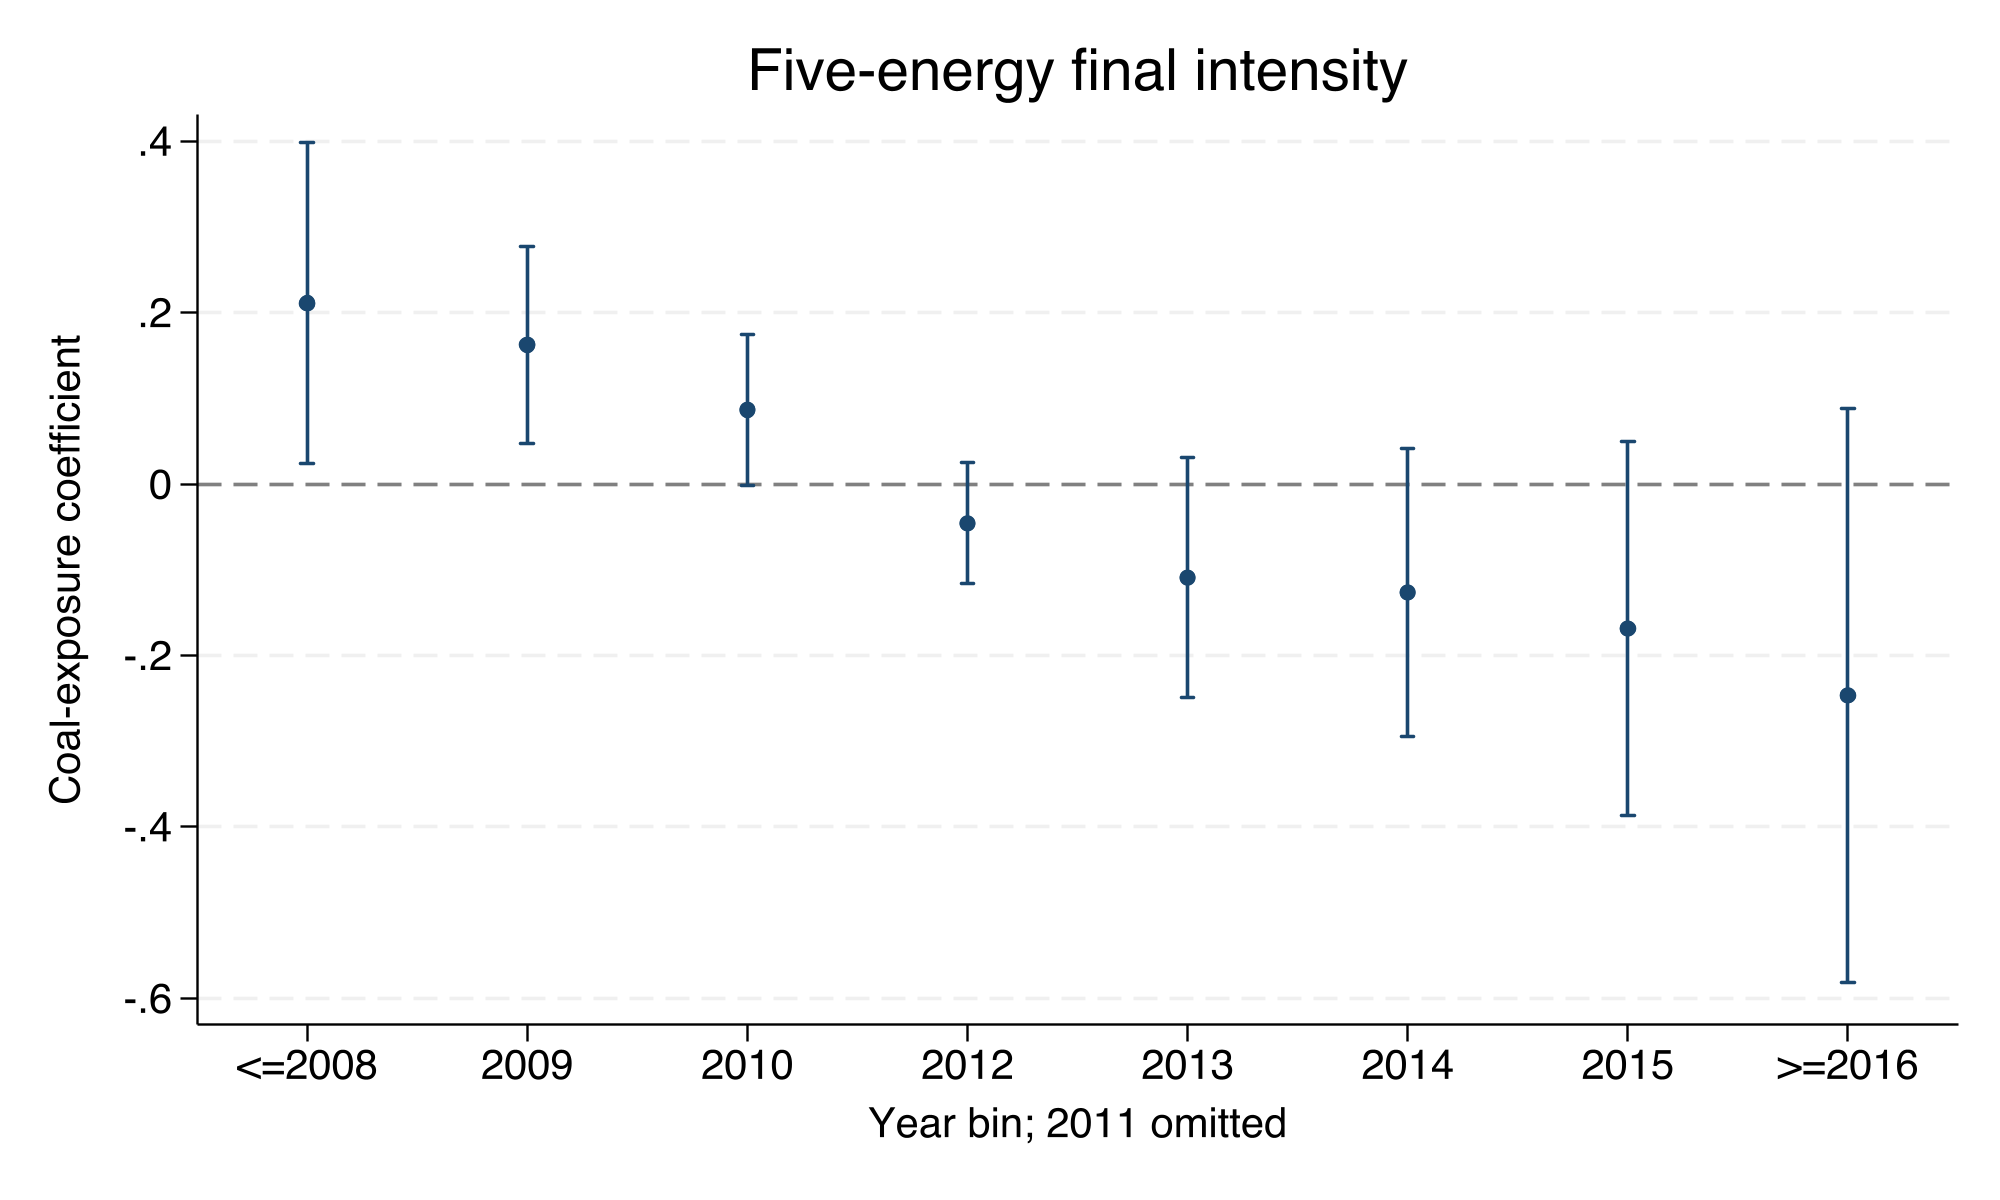
\includegraphics[width=\linewidth]{../result/figures/0718_manuscript_revision/EventStudy_energy5_int.png}
\caption{Five-energy final intensity}
\end{subfigure}
\begin{subfigure}{0.49\textwidth}
\centering
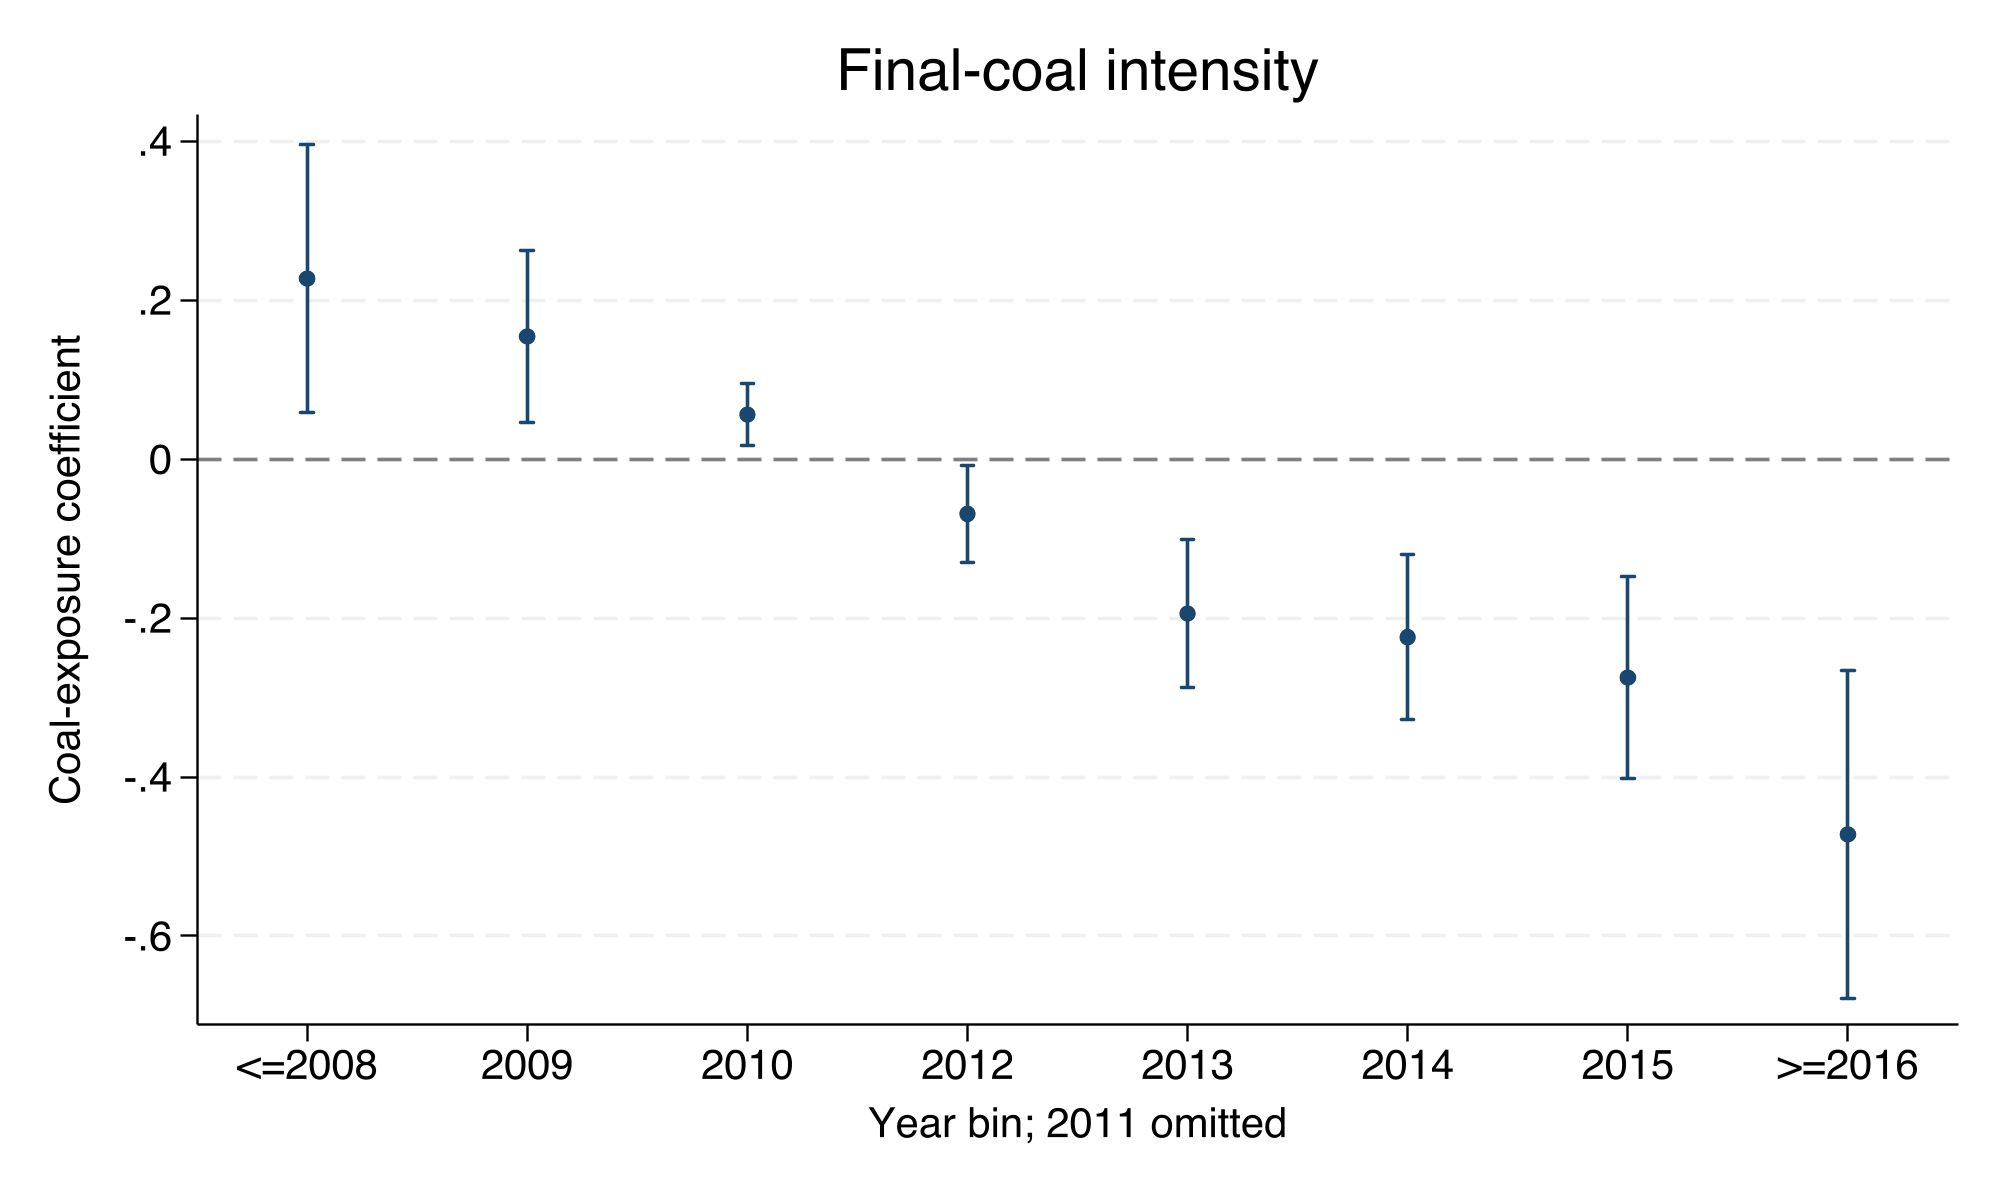
\includegraphics[width=\linewidth]{../result/figures/0718_manuscript_revision/EventStudy_coalterm_int.png}
\caption{Final-coal intensity}
\end{subfigure}

\begin{subfigure}{0.49\textwidth}
\centering
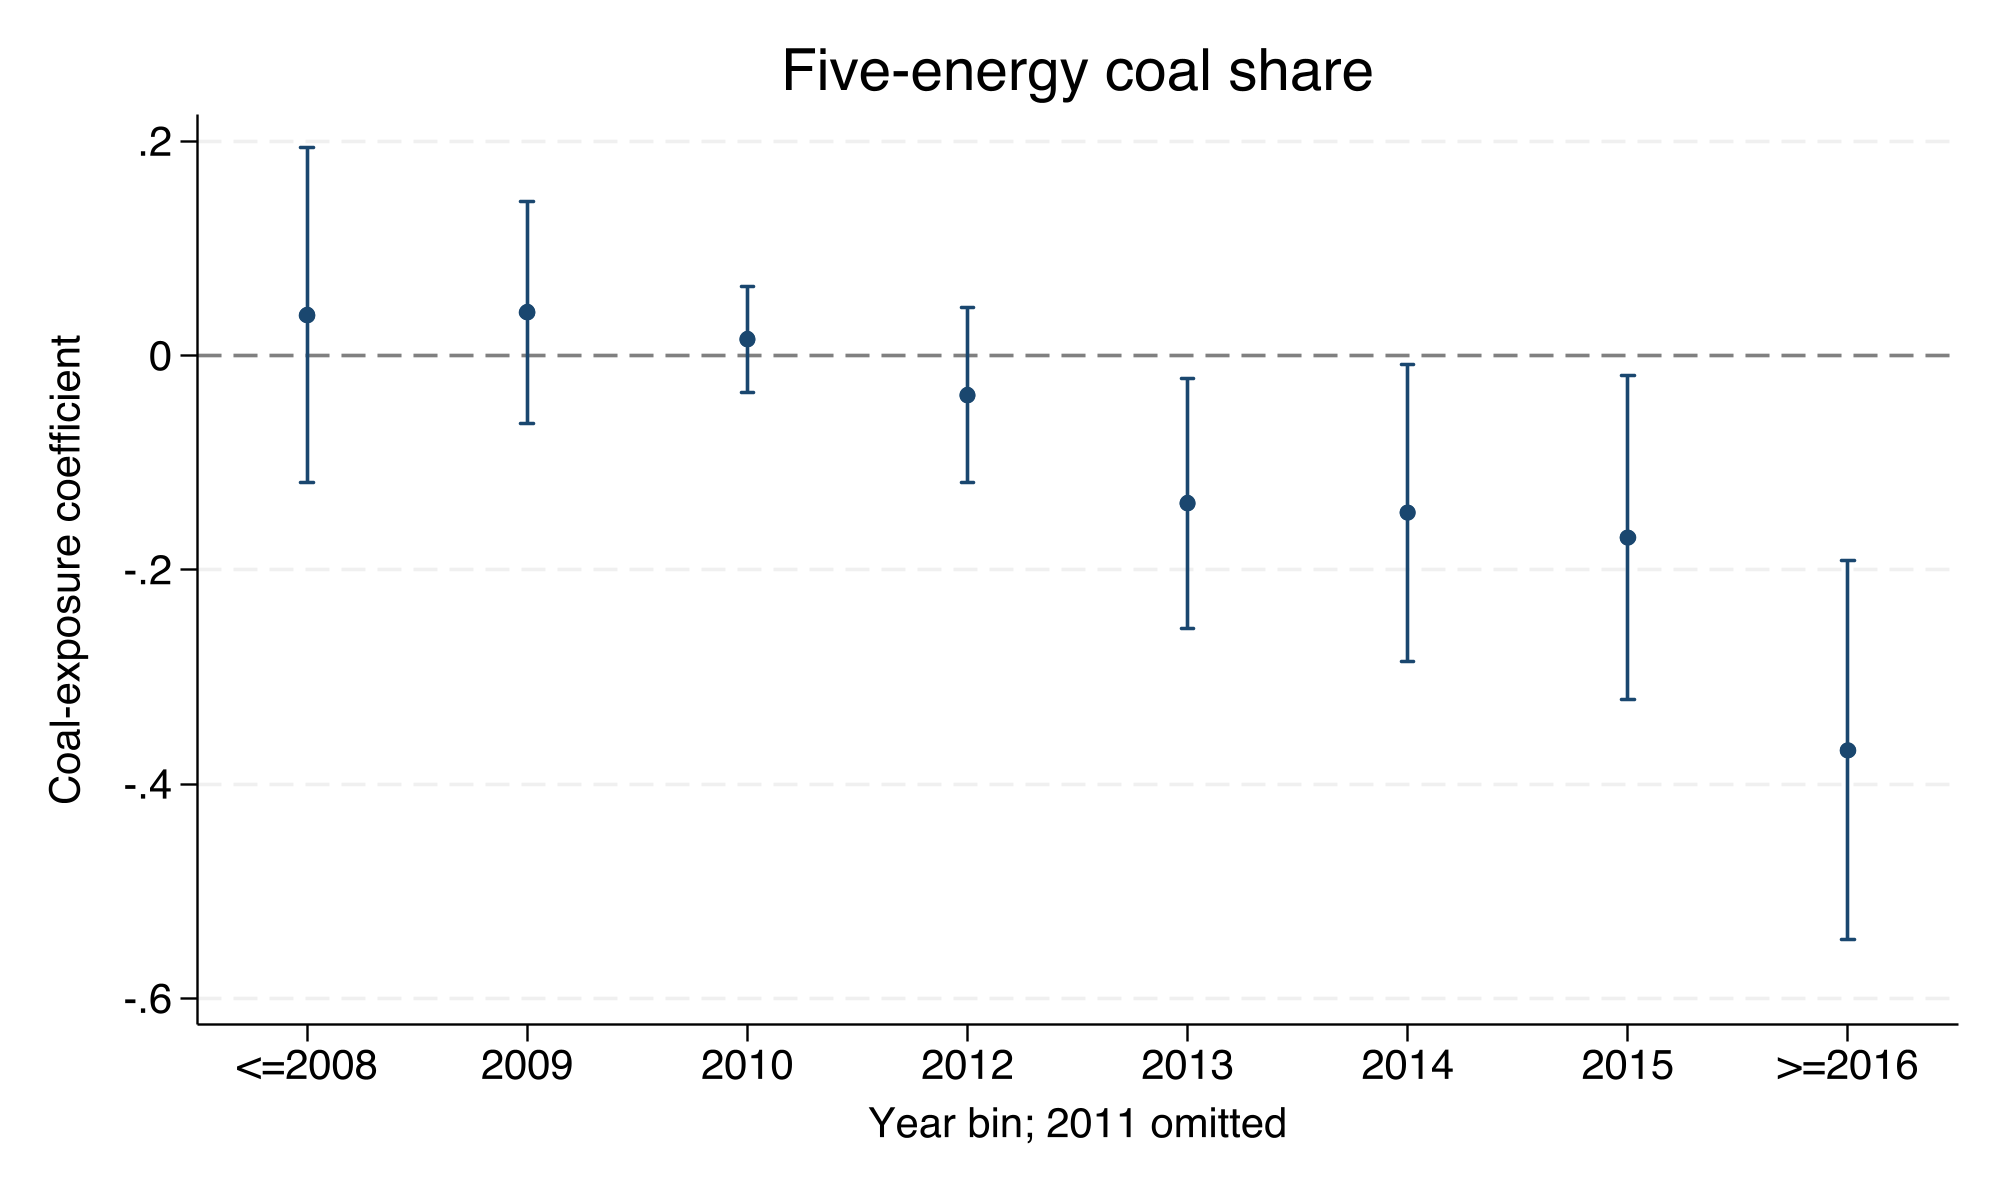
\includegraphics[width=\linewidth]{../result/figures/0718_manuscript_revision/EventStudy_coalshare5.png}
\caption{Five-energy coal share}
\end{subfigure}
\begin{subfigure}{0.49\textwidth}
\centering
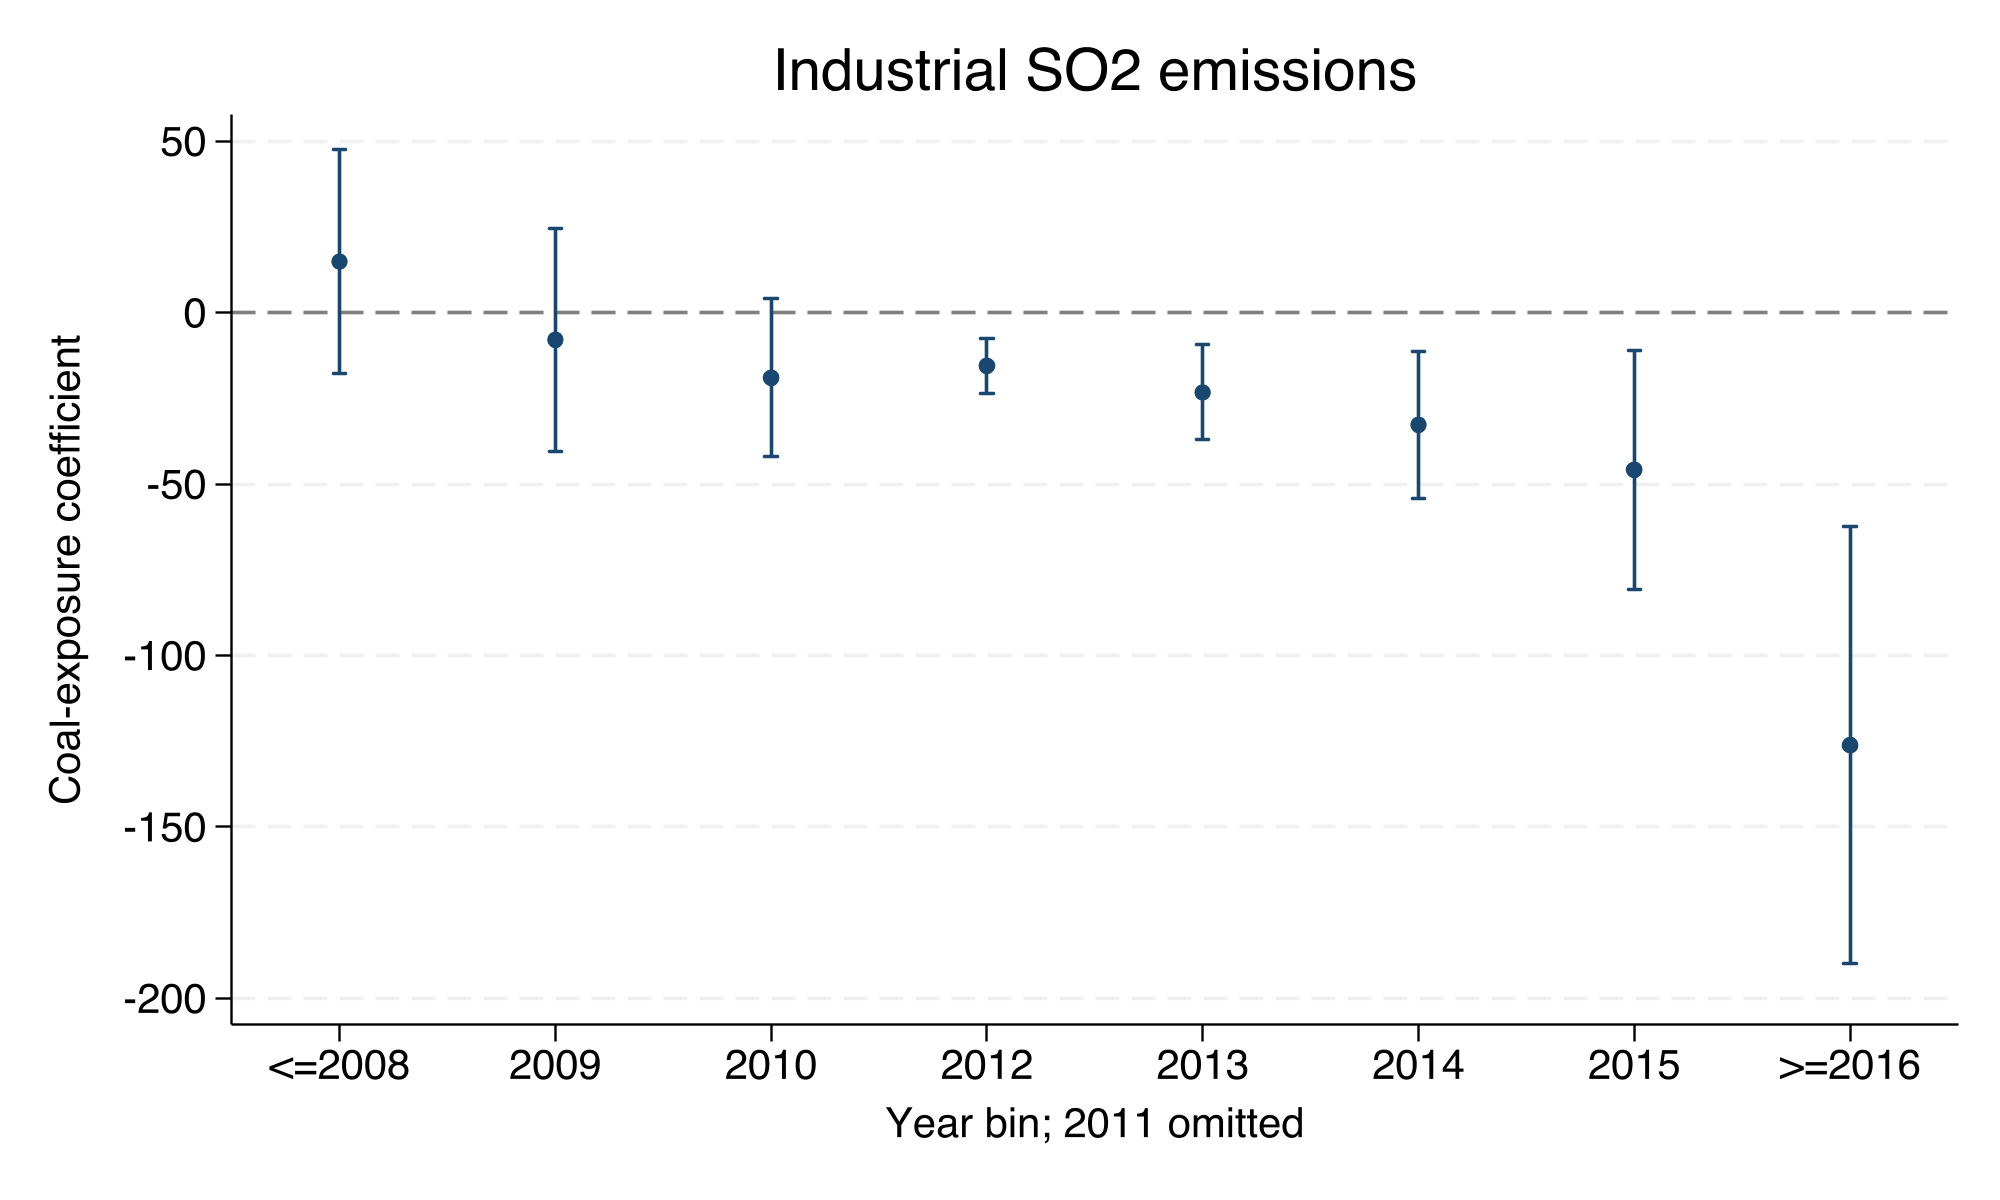
\includegraphics[width=\linewidth]{../result/figures/0718_manuscript_revision/EventStudy_industrial_so2.png}
\caption{Industrial SO$_2$}
\end{subfigure}
\caption{Continuous coal-exposure event studies}
\label{fig:event}
\note{The omitted year is 2011. The left endpoint pools 2008 and earlier; the right endpoint pools 2016 and later. Error bars are 95 percent confidence intervals.}
\end{figure}

\section{Supplementary diagnostics and data coverage}

\begin{table}[H]
\centering
\caption{Financial-side diagnostics using the green-credit proxy}
\begin{tabular}{lrrr}
\toprule
Model/outcome & Coefficient & Std. error & $p$-value \\
\midrule
Post-policy coal exposure $\rightarrow$ Green-credit proxy & 0.0809 & 0.0948 & 0.401 \\
Excluding 2017 & 0.0810 & 0.0913 & 0.382 \\
Green-credit proxy $\rightarrow$ Five-energy intensity & -0.0071 & 0.0124 & 0.568 \\
Green-credit proxy $\rightarrow$ Final-coal intensity & -0.0129 & 0.0116 & 0.277 \\
Green-credit proxy $\rightarrow$ Industrial SO$_2$ & 0.0379 & 3.6752 & 0.992 \\
Green-credit proxy $\rightarrow$ Coal share & -0.0145 & 0.0112 & 0.207 \\
Green-credit proxy $\rightarrow$ Log CO$_2$ & -0.0246 & 0.0121 & 0.052 \\
Green-credit proxy $\rightarrow$ Wind-solar generation & 0.0057 & 0.0047 & 0.234 \\
\bottomrule
\end{tabular}
\note{All models include province and year fixed effects and the baseline controls. These are correlational diagnostics.}
\end{table}

\begin{table}[H]
\centering
\caption{Temporal coverage of local infrastructure variables}
\begin{tabular}{lrrr}
\toprule
Variable & First year & Last year & Province-years \\
\midrule
Interprovincial electricity exports, Jan.--Nov. & 2015 & 2023 & 277 \\
Wind utilization hours & 2018 & 2023 & 186 \\
Solar utilization hours, Jan.--Nov. & 2018 & 2023 & 186 \\
Wind utilization/curtailment rate & 2020 & 2023 & 124 \\
Solar utilization/curtailment rate & 2020 & 2023 & 124 \\
\bottomrule
\end{tabular}
\note{Every series begins after 2012 and therefore cannot serve as a pre-policy condition in the national design.}
\end{table}

\printbibliography[title={References}]

\end{document}
